% ------------------------------------------------------------
% ------------------------------------------------------------
  
% Insert the common KETCube AppNote Defines

% ------------------------------------------------------------
% ------------------------------------------------------------

\documentclass[twoside,a4paper]{refart}
\usepackage[utf8x]{inputenc}
%\usepackage[czech]{babel}
\usepackage[pdftex]{graphicx}
\usepackage{caption}% for \captionof
\usepackage{mwe}% contains example-image
% Definition of shortcuts for authornames
%  Sort alphabetically by surname

\newcommand{\JB}{Jan Bělohoubek}
\newcommand{\JC}{Jiří Čengery}
\newcommand{\JF}{Jaroslav Freisleben}
\newcommand{\PK}{Petr Kašpar}
\newcommand{\MU}{Matin Úbl}
\newcommand{\KV}{Kryštof Vaněk}
\newcommand{\JZ}{Jan Záruba}
\newcommand{\TP}{Tomáš Pokorný}

\usepackage[owncaptions]{vhistory}
\usepackage{hyperref}
%\usepackage[superscript,biblabel]{cite}
\usepackage{multirow}
\usepackage{wrapfig}
\usepackage{float}

\usepackage[table, x11names]{xcolor}
\usepackage{fancyvrb}
\usepackage{fontawesome}
\usepackage[many]{tcolorbox}
\usepackage{listings}
\usepackage{tikz}
\usepackage{verbatimbox}

\usepackage{array, booktabs, boldline} %
\usepackage{mathtools}

\pdfinfo
{
  /Title       (The KETCube Project AppNote)
  /Creator     (LaTeX)
  /Author      (The SmartCAMPUS Team)
}

% declare the path(s) where your graphic files are
% extract presenattion number to create include path for images
\ExplSyntaxOn
% Save a copy of \jobname
\tl_set:NV \NUMBER \c_sys_jobname_str
\regex_replace_once:nnN { [A-Za-z]*_[A-Za-z]*_ } { } \NUMBER
\ExplSyntaxOff

% declare the path(s) where your graphic files are
%\graphicspath{{resources/images/}{resources/appNotes/001/images/}}
\graphicspath{{resources/images/}{resources/appNotes/\NUMBER/images/}}
\graphicspath{{resources/images/}{resources/appNotes/003/images/}}

\newsavebox{\tempbox}
\newlength{\tempheight}

\newcommand\ToDo[1]{\textcolor{red}{ToDo: #1}}

\newcommand\docNote[1]{
\subsubsection*{~\hspace{0.2cm}\textcolor{cyan}{\Huge \faCommentingO\,}}
\vspace{-1.5cm}
\begin{tcolorbox}[breakable,colback=white,colframe=cyan,width=\dimexpr\textwidth+32mm\relax,enlarge left by=-32mm, title = Note]
\it \small #1
\end{tcolorbox}
}

\newcommand\docWarn[1]{
\subsubsection*{~\hspace{0.2cm}\textcolor{orange}{\Huge \faWarning\,}}
\vspace{-1.5cm}
\begin{tcolorbox}[breakable,colback=white,colframe=orange,width=\dimexpr\textwidth+32mm\relax,enlarge left by=-32mm, title = Warning]
\it #1
\end{tcolorbox}
}

\newcommand\docExample[1]{
\subsubsection*{~\hspace{0.2cm}\textcolor{gray}{\Huge \faCogs\,}}
\vspace{-1.5cm}
\begin{tcolorbox}[breakable,colback=white,colframe=gray,width=\dimexpr\textwidth+32mm\relax,enlarge left by=-32mm, title = Example]
#1
\end{tcolorbox}
}


\newenvironment{docCodeExample}
{
\subsubsection*{~\hspace{0.2cm}\textcolor{gray}{\Huge \faCogs\,}}
\vspace{-1.5cm}
\begin{tcolorbox}[breakable,colback=white,colframe=gray,width=\dimexpr\textwidth+32mm\relax,enlarge left by=-32mm, title = Example]
}
{
\end{tcolorbox}
}

\newenvironment{docCodeListing}
{
\subsubsection*{~\hspace{0.2cm}\textcolor{cyan}{\Huge \faStickyNoteO\,}}
\vspace{-1.5cm}
\begin{tcolorbox}[breakable,colback=white,colframe=cyan,width=\dimexpr\textwidth+32mm\relax,enlarge left by=-32mm, title = Listing]
}
{
\end{tcolorbox}
}

\newcommand\docFileName[1]{{\tt #1}}
\newcommand\docVarName[1]{{\tt #1}}

%skryt barevny obdelnik kolem odkazu
\hypersetup{
    colorlinks=false,
    pdfborder={0 0 0},
}

% vhistory
\renewcommand{\vhhistoryname}{Revision History}
\renewcommand{\vhchangename}{Note}
\renewcommand{\vhversionname}{Revision}
\renewcommand{\vhdatename}{Date}
\renewcommand{\vhauthorname}{Author}
\renewcommand \vhAuthorColWidth{0.8\hsize}
\renewcommand \vhChangeColWidth{1.2\hsize}

\DeclareRobustCommand{\UWBLogo}{%
   \begin{wrapfigure}{l}{2.1cm}
    \vspace{-1.35cm}
    \includegraphics[width=2cm]{ZCU_logo.pdf}
   \end{wrapfigure}
}


\title{\UWBLogo KETCube AppNote 008:\\ KETCube Bootloader (\vhCurrentVersion)}

\author{Author: \vhListAllAuthorsLongWithAbbrev}
\date{Version \vhCurrentVersion\ from \vhCurrentDate}

% ------------------------------------------------------------
% ------------------------------------------------------------
  
% Insert the common KETCube AppNote Head

% ------------------------------------------------------------
% ------------------------------------------------------------

\begin{document}
\pagenumbering{roman} 

\titlepage
\maketitle

% ------------------------------------------------------------
% ------------------------------------------------------------
  
% BEGIN of the KETCube appNote Content

% ------------------------------------------------------------
% ------------------------------------------------------------


% ------------------------------------------------------------
% ------------------------------------------------------------
  
% BEGIN of the KETCube appNote Content

% ------------------------------------------------------------
% ------------------------------------------------------------

\section*{KETCube Bootloader: the STM Bootloader Re-Invented}
{\it KETCube} \cite{ZCU:KETCube:05-2018} is the prototyping and demo platform developed at the Department of Technologies and Measurement (KET), University of West Bohemia in Pilsen. 


This document describes the KETCube Bootloader. The bootloader is protocol-compatible with the standard ROM STM32 bootloader \cite{STM32:AN3155}. It was designed to provide a customizable bootloader with security features for the KETCube platform compatible with the standard toolset.

\setcounter{tocdepth}{2}
\tableofcontents
\clearpage

\listoffigures
\listoftables
\begin{versionhistory}
  \vhEntry{0.2.0*}{8.11.2021}{JB|KV}{Initial version}
\end{versionhistory}
% history table ... do not number
\setcounter{table}{0}

\clearpage 
\pagenumbering{arabic} 
\pagestyle{headings} 

\clearpage
\section{Bootloader Architecture} \label{sec:arch}

\marginlabel{\captionof{figure}{Bootloader operation sequence}\label{fig:bootOp:sequence}}
\raisebox{-\height}{\scalebox{0.7}{\begin{tikzpicture}[font=\small,thick]
 
\node[draw,
    rounded rectangle,
    minimum width=3.5cm,
    minimum height=1cm,
    align=center
] (block0) { Start Bootloader };
 
\node[draw,
    diamond,
    below=of block0,
    minimum width=3.5cm,
    minimum height=1cm,
    align=center
] (block1) { 0x7F or command received\\in the time window\footnotemark\\on supported interface };

\node[draw,
    below=of block1,
    minimum width=3cm,
    minimum height=1cm,
    align=center
] (block2) { USART1 selected };

\node[draw,
    below=of block2,
    minimum width=3cm,
    minimum height=3cm,
    align=center
] (block3) { Auto-baud rate sequence\\send ACK byte \& disable\\unused peripherals\footnotemark };

\node[coordinate,below=1cm of block3] (blockCmdWait) {};

\node[draw,
    diamond,
    below=1cm of blockCmdWait,
    minimum width=3cm,
    minimum height=2cm,
    align=center
] (block4) { Wait for a\\command };
 
\node[coordinate,below=1cm of block4] (blockCmdRecv) {};

\node[draw,
    below=of blockCmdRecv,
    minimum width=3cm,
    minimum height=2cm,
    align=center
] (block6) { Basic Commands\\(Get, Read, Write, \dots) };

\node[draw,
    right=of block6,
    minimum width=3cm,
    minimum height=2cm,
    align=center
] (block7) { GO cmd\\routine };

\node[below=1cm of block7, fill=white] (blockJumpAddr) {Jump To Address};
\node[right=of blockJumpAddr, fill=white] (blockJumpApp) {Jump To Application};

\node[coordinate,below=1cm of block6] (blockCmdExec) {};
\node[coordinate,below=1cm of blockCmdExec] (blockCmdExec2) {};
\node[coordinate,left=5cm of blockCmdExec2] (blockCmdExec3) {};
 
% Arrows
\draw[-latex] (block0) edge (block1)
              (block2) edge (block3)
              (block3) -- (blockCmdWait)
              (blockCmdWait) -| (block4)
              (block4) edge (blockCmdRecv);
              
\draw[->] (block1) -- (block2) node [pos=0.5,right,font=\footnotesize] { Yes };
\draw[->] (block1) -| (blockJumpApp) node [pos=0.1,above,font=\footnotesize] { No };
              
\draw[->] (blockCmdRecv) -| (block6);
\draw[->] (blockCmdRecv) -| (block7);

\draw[] (block6) |- (blockCmdExec);
\draw[->] (block7) -- (blockJumpAddr);

\draw[] (blockCmdExec) |- (blockCmdExec2)
        (blockCmdExec2) |- (blockCmdExec3);
\draw[->] (blockCmdExec3) |- (blockCmdWait);
 
\end{tikzpicture}}}
\addtocounter{footnote}{-1}
\footnotetext{The dafault time window for 0x7F reception is 5 seconds}
\addtocounter{footnote}{+1}
\footnotetext{Autobaudrate is currently NOT supported by this bootloader}

\clearpage
\subsection{Bootloader Structure and Module Dependencies}

\begin{figure}[H]
	\hspace{-3cm}
	\includegraphics[width=0.6\paperwidth]{resources/appNotes/008/modules.pdf}
\end{figure}

\clearpage
\subsection{Memory maps}\label{sec:arch:memMaps}
\subsubsection{Program Flash Memory Map} \label{sec:arch:flashMap}

\marginlabel{\captionof{figure}{Program Flash}\label{fig:arch:flashMap}}
\raisebox{-\height}{

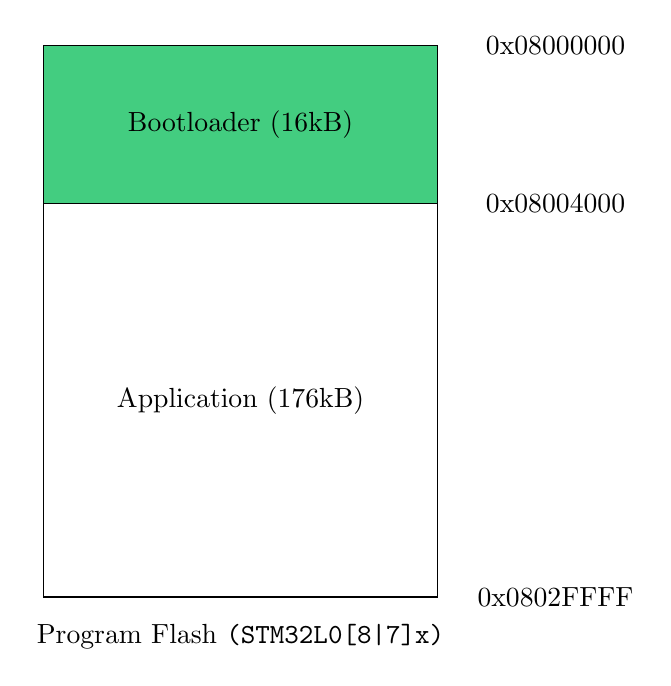
\begin{tikzpicture}
  \node[draw,fill=white,    minimum height=5cm,minimum width = 5cm,yshift=0cm](10/5){Application (176kB)};
  \node[draw,fill=SeaGreen3,minimum height=2cm,minimum width = 5cm,yshift=3.5cm](10/5){Bootloader (16kB)};
  
  \node[anchor=center,yshift=4.5cm,xshift=4cm,fill=white] {0x08000000};
  \node[anchor=center,yshift=2.5cm,xshift=4cm,fill=white] {0x08004000};
  \node[anchor=center,yshift=-2.5cm,xshift=4cm,fill=white] {0x0802FFFF};
  
  \node[anchor=center,yshift=-3.0cm,xshift=0cm,fill=white] {Program Flash \texttt{(STM32L0[8|7]x)}};
\end{tikzpicture}
}

\subsubsection{Volatile Data Memory Map} \label{sec:arch:RAMMap}

\marginlabel{\captionof{figure}{Volatile Memory (RAM)}\label{fig:arch:RAMMap}}
\raisebox{-\height}{

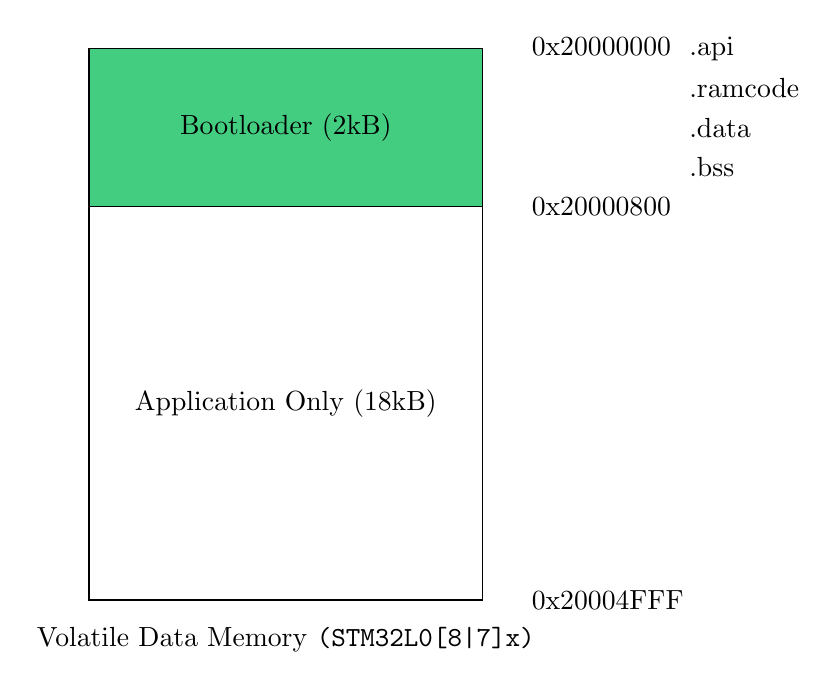
\begin{tikzpicture}
  \node[draw,fill=white,    minimum height=5cm,minimum width = 5cm,yshift=0cm](10/5){Application Only (18kB)};
  \node[draw,fill=SeaGreen3,minimum height=2cm,minimum width = 5cm,yshift=3.5cm](10/5){Bootloader (2kB)};
  
  \node[anchor=west,yshift=4.5cm,xshift=3cm,fill=white]  {0x20000000~~.api};
  \node[anchor=west,yshift=4.0cm,xshift=5cm,fill=white]  {.ramcode};
  \node[anchor=west,yshift=3.5cm,xshift=5cm,fill=white]  {.data};
  \node[anchor=west,yshift=3.0cm,xshift=5cm,fill=white]  {.bss};
  \node[anchor=west,yshift=2.5cm,xshift=3cm,fill=white]  {0x20000800};
  \node[anchor=west,yshift=-2.5cm,xshift=3cm,fill=white] {0x20004FFF};
  
  \node[anchor=center,yshift=-3.0cm,xshift=0cm,fill=white] {Volatile Data Memory \texttt{(STM32L0[8|7]x)}};
\end{tikzpicture}
}

The Bootloader API object (structure of function pointers) is located at the beginning of the (Bootloader) RAM area in the \texttt{.api} section to allow straight-forward application-bootloader interfacing. 

The \texttt{.api} section is followed by the \texttt{.ramcode} section holding Bootloader code executed from RAM. 

The rest of the bootloaders' RAM is dedicated for initialized and uninitialized data (common \texttt{.data} and \texttt{.bss} sections).

\docNote{RAM used by the bootloader cannot be re-used by Application. 

Application \textbf{must not} use memory reserved for bootloader!}


\clearpage
\subsection{Non-Volatile Data Memory Organization} \label{sec:arch:EEPROMMap}

The microcontroller Non-Volatile Memory (NVM) is typically organized in one or more banks.
The typical EEPROM memory organization with two banks is shown in Figure~\ref{fig:arch:EEPROMMap}.

\docNote{Our default targets (\texttt{(STM32L0[8|7]x)}) are quit typical and employ two EEPROM Banks.}

\marginlabel{\captionof{figure}{Physical\\EEPROM Organization}\label{fig:arch:EEPROMMap}}
\raisebox{-\height}{

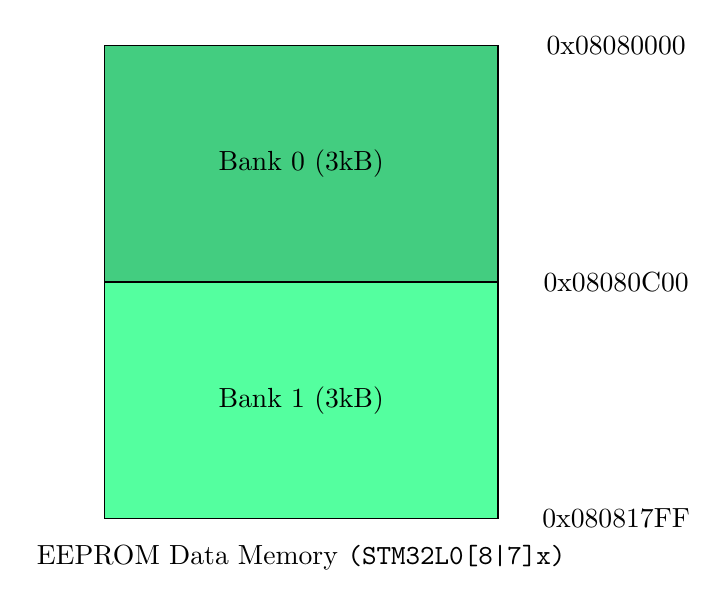
\begin{tikzpicture}
  \node[draw,fill=SeaGreen1,    minimum height=3cm,minimum width = 5cm,yshift=0cm](10/5){Bank 1 (3kB)};
  \node[draw,fill=SeaGreen3,minimum height=3cm,minimum width = 5cm,yshift=3cm](10/5){Bank 0 (3kB)};
  
  \node[anchor=center,yshift=4.5cm,xshift=4cm,fill=white]  {0x08080000};
  \node[anchor=center,yshift=1.5cm,xshift=4cm,fill=white]  {0x08080C00};
  \node[anchor=center,yshift=-1.5cm,xshift=4cm,fill=white] {0x080817FF};
  
  \node[anchor=center,yshift=-2.0cm,xshift=0cm,fill=white] {EEPROM Data Memory \texttt{(STM32L0[8|7]x)}};
\end{tikzpicture}
}

The NVM could be used as a linear address space or independent memory banks could be employed e.g. for concurrent read/write access.
In our case, the independent banks are unused or used to increase data diversity depending on the bootloader configuration. 

\subsubsection{Logical NVM Organization}\label{sec:arch:EEPROMMap:logical}

To increase the reliability of the storage and to distribute EEPROM writes load equally, the bootloader employs the logical layer above the physical non-volatile memory (NVM). 
The logical layer decreases the effective size of NVM while increasing the NVM storage reliability and durability. 

Data in the non-volatile memory (NVM) are hold in \textit{blocks}. Blocks employ a mechanism of data versioning, 
and the recent valid block only is available, while the other blocks serve as backup blocks. The Block structure is shown in Figure \ref{fig:arch:Block}. 

\marginlabel{\captionof{figure}{Logical NVM Organization -- block structure}\label{fig:arch:Block}}
\raisebox{-\height}{

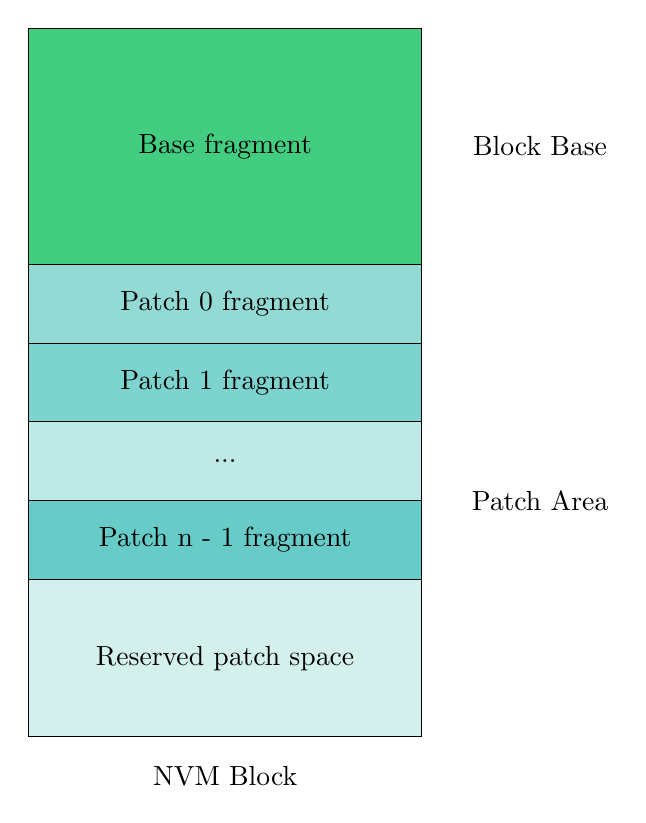
\begin{tikzpicture}
  \node[draw,fill=White,    minimum height=7cm,minimum width = 5cm,yshift=0cm](10/5){};
  \node[draw,fill=SeaGreen3,minimum height=3cm,minimum width = 5cm,yshift=3cm](10/5){Base fragment};
  \node[draw,fill=BlueGreen!50!,    minimum height=1cm,minimum width = 5cm,yshift=1cm](10/5){Patch 0 fragment};
  \node[draw,fill=BlueGreen!60!,    minimum height=1cm,minimum width = 5cm,yshift=0cm](10/5){Patch 1 fragment};
  \node[draw,fill=BlueGreen!30!,    minimum height=1cm,minimum width = 5cm,yshift=-1cm](10/5){ ... };
  \node[draw,fill=BlueGreen!70!,    minimum height=1cm,minimum width = 5cm,yshift=-2cm](10/5){Patch n - 1 fragment};
  \node[draw,fill=BlueGreen!20!,    minimum height=2cm,minimum width = 5cm,yshift=-3.5cm](10/5){Reserved patch space};
  
  \node[anchor=center,yshift=3.0cm,xshift=4cm,fill=white]  {Block Base};
  \node[anchor=center,yshift=-1.5cm,xshift=4cm,fill=white]  {Patch Area};
  
  \node[anchor=center,yshift=-5.0cm,xshift=0cm,fill=white] {NVM Block};
\end{tikzpicture}
}

Each NVM block is composed of two main areas: the \textit{Block Base} and the \textit{Patch Area}. 
Data itself are held in simple containers called \textit{fragments}. NVM contains one or more blocks.

The \textit{Block Base} area holds a single fragment called \textit{base fragment}. 
The \textit{base fragment} represents an effective size of the NVM block, while its default size is 1kB.
The \textit{base fragment} represents a plain memory containing the NVM block data in a conventional way.

The \textit{Patch Area} holds multiple fragments called \textit{patch fragments}.
The default \textit{Patch Area} size is 0.5kB, while the \textit{patch fragment} size is variable.
Each \textit{patch fragment} holds a patch related to the \textit{base fragment} and previous \textit{patch fragments}.
By applying valid patches sequentially to data hold in the \textit{base fragment}, 
the NVM block content is recovered.

Each \textit{fragment} is composed of the fixed-size header and data. The fragment header format is as follows:

\begin{table*}[!ht]
  \hspace*{0cm}
  \begin{tabular}{| p{5cm} | p{5.5cm} | }
      \hline
      \rowcolor{SeaGreen3!30!} {\bf Field} & {\bf Description} \\
      \hline
      \hline
      {\tt cfg     } ({\tt uint32\_t}) \newline bitfield  & {\tt 0x00000000} -- Base Fragment;\newline
                          {\tt 0x00000001} -- Patch Fragment;\newline
                          {\tt others} -- RFU\\
      \hline
      {\tt version } ({\tt uint32\_t }) & fragment age/version \newline {\tt [1, INT\_MAX]}\\
      \hline
      {\tt offset  } ({\tt uint16\_t })  & Fragment data offset in the block \\
      \hline
      {\tt length  } ({\tt uint16\_t })  & Fragment data length \\
      \hline
      {\tt crc32   } ({\tt uint32\_t })  & Fragment header and data checksum \\
      \hline
  \end{tabular}
  \addcontentsline{lot}{table}{NVM Fragment Header}
  \label{tab:nvmFragmentHeader}
 \end{table*}

\clearpage
 \docNote{Fragment versions in a single NVM Block is the uninterrupted rising series of integers (incremented by one). In case of a gap (> 1) between the following version numbers, the next fragment is considered invalid.}
 
 \docNote{Note, that there is no need to reset the fragment version field or watch for overflow, because 32-bit version field allows to represent more than 10M of full 6kB EEPROM writes (in the pessimistic case, for the smallest possible fragments), which is much above typical EEPROM durability.}

 \docNote{Fragment version field represents the utilization of the memory and if the memory was not completely erased, it might serve as a memory age indicator.}
 
\subsubsection{Failsafe Features}\label{sec:arch:EEPROMMap:failsafe} 
 
 Depending on the bootloader configuration, the physical memory is used logically as a single-bank memory or as a dual-bank mirrored memory with half capacity. 

\docWarn{The dual-bank mirrored case is not implemented yet.}
 
 In the single-bank case, the capacity of the memory is higher allowing more blocks could be stored in NVM. 
 If memory content is damaged during a write operation, only the latest fragment is damaged. 
 As fragments employ the self-checking CRC32 mechanism for error-detection, an error is discovered when EEPROM is read and automatic rollback to the previous patch/block is performed.

 In the mirrored memory organization, blocks are synchronously stored in both banks to increase the diversity of data. 
 In case of inconsistency, read/write operations in dual-bank arrangement select the newer valid content from both banks and initiate damaged bank recovery.
 If memory content is damaged during write, no rollback is taken, but the second memory bank content is used to recover recent data and restore consistency.
 
\docWarn{If an EEPROM cell is permanently damaged, the current implementation in the single-bank case is unable to recover - no new patches could be stored.
On the other hand, in the dual-bank case, the undamaged bank could be used exclusively.}
 
\subsubsection{Security Features}\label{sec:arch:EEPROMMap:sec}

The NVM memory could be protected by standard MCU read-out protection mechanism and by access priviledge mechanism implemented in KETCube bootloader.


\clearpage
\section{Supported Devices}\label{sec:supportedDevices}

\docNote{This bootloader is designed to be generic, however, it is currently tested only on STM32L0[7|8][1-3] devices.}

\subsection{STM32L0[7|8][1-3]}

\subsubsection{Clock Configuration}
The primary clock source is PLLCLK at 32 MHz, derived from HSI (RC clock, crystal-less).

\subsubsection{Watchdog}
Independent watchdog (IWDG) is currently not handled by the bootloader -- please note, that, it might cause problems if IWDG is enabled by application.


\subsection{Adding a New Device}

To add a new device:
\begin{enumerate}
\item insert the device definitions to the \docFileName{device.h} file, 
\item create the custom memory map in the \docFileName{memory} directory and include it to the linker script \docFileName{LinkerScript.ld},
\item re-visit or re-implement the \docVarName{dev\_initClock()} function,
\item re-visit or re-implement the interface implementation(s)\\in~\docFileName{iface\_IFACE.c},
\item re-visit or re-implement and verify the TRNG module.
\end{enumerate}

For the STM32 devices specification details, see Table 149 in \cite{STM32:AN2606}.

Always use the preprocessor conditional expressions, conditional block, or conditional includes to add a new device, e.g. \docVarName{\#if defined(STM32L071xx)} 

\begin{docCodeExampleTitled}{Conditional Include of SPI Interface Handler for STM32L071xx}
\begin{verbatim}
#if defined(STM32L071xx) 
#include "iface_spi_stm32l071xx.c"
#endif
\end{verbatim}
\end{docCodeExampleTitled}

\docNote{To select the device, set \docVarName{DEVICE} variable in the Makefile to the device-speciffic string, e.g. to \docVarName{STM32L071xx} to select STM32l071 device.}

\clearpage
\section{Supported Interfaces}

\subsection{Default Interface: UART}

Configuration for the KETCube bootloader default target:
\begin{itemize}
  \item peripheral: UART1
  \item Tx PIN: PA9
  \item Rx PIN: PA10
  \item Default Baud Rate: 57600 bps
  \item Data bits: 8
  \item Stop bits: 1
  \item Parity: Even
  \item HW Flow control: No
\end{itemize}

\docNote{The auto-baud rate feature implemented by the standart STM bootloader is currently not implemented in KETCube bootloader.}

\subsection{Adding New Interface}

To add a new interface support:
\begin{enumerate}
\item implement the interface handler \docFileName{iface\_IFACE.c}\footnote{IFACE should represent a well-known abbreviation of the interface} implementing the \docFileName{iface.h} API,
\item modify the \docFileName{iface.c} file to conditionally include \docFileName{iface\_IFACE.c}.
\end{enumerate}

\clearpage
\section{Bootloader Configuration} \label{sec:settings}

Bootloader is written to be compile-time and run-time configurable. 
The compile-time configuration is realized through preprocessor defines, as described below.
To store the run-time configuration, this bootloader uses a portion of NVM.
Altering the run-time configuration is possible through the application API 
or through special commends through standard bootloader protocol.

\subsection{Build System}

KETCube bootloader utilizes the standard \docVarName{Makefile}-centric build process automation. 

\docVarName{Doxygen} is used for code-level documentation and requirement tracking.

The Arm GNU Toolchain (\docVarName{GCC}) is currently the only supported compiler.


\subsection{Custom Build Configuration}

  The folowing table summarizes the compile- and link-time options, which can be used for the static bootloader configuration.

  \begin{table*}[!ht]
    \hspace*{-4cm}
    \begin{tabular}{| p{5.5cm} | p{7.5cm} |}
        \hline
        \rowcolor{SeaGreen3!30!} {\bf Option} & {\bf Description} \\
        \hline
        \hline
        \texttt{ACCESS\_ENABLE\_PASSWORD} & Enable password to unlock the bootloader \\
        \hline
        \texttt{AES\_128\_OTFK} & USE AES 128 only, On-the-fly \\
        \hline
        \texttt{AES\_128\_PREKEYED} & USE AES 128 only, Prekeyed \\
        \hline
        \texttt{CMD\_ENABLE\_ERASE\_MEM} & Enable the deprecated erase memory command \\
        \hline
        \texttt{IFACE\_UART} & Use UART interface\\
        \hline
        \texttt{IFACE\_I2C} & Use I2C interface - NOT Implemented yet!\\
        \hline
        \texttt{IFACE\_UART\_BR\_115200} & UART interface baudRate is 115200, default is 57600\\
        \hline
        \texttt{IFACE\_UART\_PARITY\_NONE} & UART interface parity is NONE, default is EVEN\\
        \hline
        \texttt{IFACE\_UART\_MAX\_BYTE\_TIMEOUT} & UART maximum timeout for sinle byte Rx\\
        \hline
        \texttt{TESTS\_ENABLE} & All test commands are enabled and linked\\
        \hline
        \texttt{TEST\_FORCE\_UNLOCK} & Bootloader is unlocked permanently \\
        \hline
    \end{tabular}
    \addcontentsline{lot}{table}{Bootloader Build Options}
    \label{tab:cmdset}
   \end{table*}
   
   The folowing table summarizes used weak functions, which may be re-defined by end user on project basis to afect bootloader behavior, e.g. to enable interfacing with speciffic peripherals or set-up the appliocation enviroment specifically.
   
   \begin{table*}[!ht]
    \hspace*{-4cm}
    \begin{tabular}{| p{5.5cm} | p{7.5cm} |}
        \hline
        \rowcolor{SeaGreen3!30!} {\bf Function} & {\bf Description} \\
        \hline
        \hline
        \texttt{dev\_userInit()} & function is executed after interface initialization\\
        \hline
        \texttt{dev\_userAppInit()} & function is executed before application initialization\\
        \hline
    \end{tabular}
    \addcontentsline{lot}{table}{Bootloader Weak Function Hooks}
    \label{tab:cmdset}
   \end{table*}
   
   \docNote{The typical \texttt{dev\_userInit()} use case is, that the bootloader initializes UART-to-Anything converter.}

\clearpage
\subsection{Non-Volatile Run-Time Bootloader Configuration} \label{sec:cfg:runtime}

\begin{table*}[!ht]
  \hspace*{-4cm}
  \begin{tabular}{| p{4cm} | p{9cm} | }
      \hline
      \rowcolor{SeaGreen3!30!} {\bf Type} & {\bf Description} \\
      \hline
      \hline
      {\tt startup\_t } \newline ({\tt uint16\_t })  & {\tt 0x0000} -- wait for five seconds for command, then start application if available;\newline
                          {\tt 0x0001} -- start application code immediatelly (do not enter bootloader);\newline
                          {\tt 0x0002} -- stay in bootloader until timeout;\newline 
                          {\tt 0x0003} -- stay in bootloader until go.\\
      \hline
      {\tt security\_t } \newline ({\tt uint16\_t }) & see \nameref{sec:arch:secModes}\\
      \hline
      {\tt uint32\_t}    & Application Startup Timeout in milliseconds \\
      \hline
      {\tt uint32\_t *}  & Application Code start address\newline
                           (do not jump to application if {\tt NULL}) \\
      \hline
      {\tt uint8\_t[16]} & Bootloader Password/Unlock Key\newline
                           (bootloader is unlocked if {\tt NULL}) \\
      \hline
      {\tt uint8\_t[16]} & Application Code CMAC Key \\
      \hline
      {\tt uint8\_t[16]} & Application Code Encryption Key \\
      \hline
      {\tt uint8\_t[68]} & RFU \\
      \hline
  \end{tabular}
  \addcontentsline{lot}{table}{Bootloader Configuration Structure}
  \label{tab:cfgStruct}
 \end{table*}
 
\docNote{The employed threat model states, that a running application is completely trusted by the bootloader. Application can use the bootloader configuration API to set up the bootloader. The application should write to the bootloader Non-Volatile Configuration memory using bootloader configuration API exclusively to ensure configuration correctness. Bootloader configuration API may serve, e.g. for out-of-band bootloader key management.}

\subsection{Bootloader Upgrade Procedure}
\docNote{To upgrade the Bootloader, it is currently recommended to use the ROM bootloader or SWD interface.}


\clearpage
\section{Bootloader Security} \label{sec:security}

This bootloader is designed to provide a basic level of security and trust in constrained,
low-power and low-cost devices like IoT nodes, wireless batery sensors, etc.

The primary aim of this bootloader is to control access to confidential data stored in embedded MCU memories.
Unpriviledged access thru interfaces controlled by this bootloader is prohibited if the bootloader is properly configured.

Access to embedded memories thru physical interfaces not handled by this bootloader, 
or as a result of silicon-level error is not and could not be covered by this bootloader.

It is the responsibility of the organization deploying the final application to cofigure the target MCU
in such a way to disable access channels, which may compromise the MCU security outside the bootloader like
e.g. JTAG/SWD or manufacturers' insecure bootloader.

\subsection{Attacker Model} \label{sec:security:model}

This section discusses how we modeled the vulnerabilities and how should the KETCube bootloader behave to protect confidential data if configured restrictively.

Please note, that there is an option to configure this bootloader to behave completely open and provide transparent access to all MCU resources (e.g. the TEST build, or \docVarName{ACCESS\_PRIV\_UNLOCK} security mode).¨

\subsubsection*{Attacker Has Full Access to MCU Interfaces}

The attacker has full (physical) access to the MCU and has the ability and proper tools (JTAG/SWD probe, UART cable, etc.) 
to establish an electrically valid connection to the bootloader. The attacker must not be able to read out or modify 
confidential data stored in embedded MCU memories without knowledge of a secret key or password.

Under certain (still restricted) bootloader configurations, an attacker may be able to upload its firmware to MCU, 
but the bootloader assures that confidential data have vanished from MCU before untrusted code is executed.
Depending on the underlying MCU and its features, this might lead also to bootloader code vanishing from the MCU flash.

\subsubsection*{Attacker Can Read Data Downloaded to Bootloader}

It is assumed, that an attacker may unintentionally (e.g. intercepted confidential communication) or intentionally (e.g. untrusted technician)
gain access to data intended for download to the bootloader.

Bootloader provides mechanisms to verify application prior to execution (AES-CMAC). 
If propper security mode is set, the application code signature must be verified
prior execution: untrusted application execution is not possible.

Bootloader provides the firmware encryption/decryption feature to protect firmware image -- uploading of the encrypted firmware image is possible.

\docNote{Firmware encryption/decryption feature is not implemented yet!}

The signature verification and encryption mechanisms allow that firmware upgrade could be performed by an untrusted technician, 
as the signature verification mechanisms ensure, that only verified firmware is executed, 
and the firmware encryption mechanism ensures there is no leak of the protected (confidential) firmware image.

Bootloader provides AES/TRNG key-based challenge/response protocol to allow full remote unlock of the bootloader
without providing the secret key to the third person (e.g. the technician performing MCU maintenance) -- the unlock key should not leave the secure storage.

\docNote{Bootloader initial configuration and key upload must be performed in a trusted environment, and keys must be held in secured storage only.}

\subsubsection*{Running Application Is Trusted}

The bootloader does not protect against the running application -- the running application has full trust. 
If an attacker can upload its application (thru an unsecured channel), he might take over the control over the device and all confidential content.

\subsubsection*{Attacks Targeting the Underlying MCU}

Sophisticated attack methods like side-channel or fault attacks are not and could not be handled by this bootloader,
as the countermeasures need to be implemented also at the silicon level.

\subsection{Standard MCU Security Features} \label{sec:security:mcu}
 
The typical MCU running this bootloader is employed by additional channels to access embedded memories. These channels, such as JTAG/SWD interface, 
or a custom ROM bootloader must be completely disabled or at least constrained to limit access to embedded memories: 
at least read-out protection of embedded memories must be active to guarantee the confidentiality of the content of embedded memories.

This bootloader currently does not implement any (software) side-channel attack countermeasures, 
and additionally, it was designed to be portable -- crypto functions are realized in software. If the target MCU is employed by a (protected) peripheral, 
it is recommended to extend the bootloader to utilize this peripheral instead of the default deployed software implementation. 

\subsection{Bootloader Access Control} \label{sec:security:access}

The bootloader employs a simple two-layer access control mechanism to grant access to the bootloader functions.

The root layer of the access control employs two bootloader states to grant access to bootloader functions:

\begin{itemize}
  \item \texttt{Locked State} -- in the locked state, access privileges -- see \nameref{sec:arch:secModes} below -- are used to control access to bootloader functions.
  \item \texttt{Unlocked State} -- in the unlocked state, the user has full control over the bootloader command set.
\end{itemize}

\subsubsection*{Bootloader Access Privileges and Security Mode} \label{sec:arch:secModes}

The bootloader defines the command access privileges for fine-grained access control in the locked state. 

Each command defines the access privilege level, while the bootloader settings define the bootloader security mode
(part of the NVM configuration -- see \ref{sec:cfg:runtime}) determining enabled commands. 

The bootloader security mode must at least match the specified command access privilege level to enable command execution.
Commands with lower access privileges are always enabled in higher security modes.
The following table summarizes command priviledges and bootloader security modes:

\begin{table*}[!ht]
  \hspace*{-4cm}
  \begin{tabular}{| p{4cm} | p{1.5cm} | p{8.5cm} | }
      \hline
      \rowcolor{SeaGreen3!30!} {\bf Name} & {\bf Mask} & {\bf Description} \\
      \hline
      \hline
      {\tt ACCESS\_PRIV\_UNLOCK} & {\tt 0x0000} & Not restricted, commands are always enabled.\\
      \hline
      {\tt ACCESS\_PRIV\_INFO} & {\tt 0x0001} & Informative commands, bootloader and MCU information could be read-out.\\
      \hline
      {\tt ACCESS\_PRIV\_WRITE} & {\tt 0x0003} & Memory write commands, write to application memory areas is allowed, while running unverified code is not allowed.\\
      \hline
      {\tt ACCESS\_PRIV\_READ} & {\tt 0x0007} & Memory read commands, readout memory is allowed.\\
      \hline
      {\tt ACCESS\_PRIV\_CONFIG} & {\tt 0x000F} & Bootloader configuration commands, bootloader configuration could be altered.\\
      \hline
      {\tt ACCESS\_PRIV\_TEST} & {\tt 0x001F} & Bootloader special test commands, bootloader tests could be executed, no test comamnds are included in the final release bootloader builds.\\
      \hline
  \end{tabular}
\end{table*}

\docNote{For priviledges lower than \docVarName{ACCESS\_PRIV\_CONFIG}, the new application could be uploaded to the application area, however, it could not be executed until it is verified by AES-CMAC. Unsigned applications could not be executed!}

\docNote{For priviledges lower than \docVarName{ACCESS\_PRIV\_CONFIG}, the bootloader configuration is write and read-out protected thru the bootloader protocol (not from the running application).}

\docNote{The bootloader security mode representation in the NVM is inverted: the empty memory implies that all privileges are granted.}
   
   
\clearpage
\section{Application Interface}

\subsection{Application Requirements}
\subsubsection*{Application MUST:}
\begin{itemize}
  \item respect the memory map defined by the bootloader and use application-only memory
\end{itemize}

\subsubsection*{Application SHOULD NOT:}
\begin{itemize}
  \item modify \docVarName{VTOR}\footnote{\docVarName{Vector Table Offset Register} -- defines the offset of the interrupt vector table in the ARM memory} register -- e.g. applications generated by STM32Cube set the \docVarName{VTOR} register to the beginnig of the flash area
  \item write to NVM beyond the bootloader API -- bootloade settings would be demaged!
\end{itemize}

\subsubsection*{Prior executing the application code, the bootloader sets:}
\begin{itemize}
  \item the application stack to the value stored at the first word of the application flash area
  \item the interrupt vector (\docVarName{VTOR}) to the beginning of the application area
\end{itemize}

\clearpage
\subsection{Bootloader API} \label{sec:api}

Bootloader provides its standard API for the application to expose its' standard configuration interface to the application,
provide standard access to NVM, and provide access to standard security primitives -- currently AES and TRNG. 
The application can benefit from available AES or TRNG modules and the application memory footprint could be decreased, which may be important, especially in constrained applications.

The bootloader API is available through the API object (a standard C, but OOP-like structure of semantically grouped function pointers) and it's defined in the \docFileName{api.h} file, which must be included in the application.

\docNote{Please note, that bootloader API functions are executed in the context of an application, thus
if the bootloader API is used by the application, the running application must provide the access to time base through the API. 
Simply said, the bootloader needs a pointer to function returning a monotonically rising (interrupt- or peripheral-read-based) number representing (approximately) running/passed milliseconds.
KETCube bootloader API functions do not disable interrupts.}

The following text will briefly describe the KETCube API modules.

\subsubsection*{AES}
Provides Access to the AES encryption function.

\subsubsection*{APP}
Allows an application to pass required application context settings to the Bootloader API 
-- currently, an only function returning a monotonically rising number representing the number of milliseconds is required (e.g. STM's standard HAL\_getTick()).

\subsubsection*{CFG}
Exposes the bootloaders' standard configuration API to the application.

\subsubsection*{NVM}
Exposes the API to access the non-volatile memory of the application.
In case, the application does not use this API to access NVM, 
the bootloader must be configured to use a limited portion of NVM,
and the application must not modify the area used by the bootloader.

\subsubsection*{TRNG}
Provides Access to the bootloaders' True Random Number Generator utilizing RC oscillator jitter.

\clearpage
\section{Cryptographic Functions}
This section summarizes information on portable (software implemented) cryptographic primitives employed by the KETCube bootloader.

\subsection{Advanced Encryption Standard (AES-128)}

The block-cipher selected for use with the bootloader is NIST standard \textit{Advanced Encryption Standard} (AES)~\cite{NIST:AES} with 128-bit block size. 

The software implementation of the AES module itself is based on third-party open-source implementation originally published by Brian Gladman from Worcester, UK.  This AES implementation is proven by several open source projects -- e.g. LoRaMac-node\footnote{\url{https://github.com/Lora-net/LoRaMac-node/tree/master/src/peripherals/soft-se}} is a reference closely related to the KETCube project. The AES module is distributed under a specific BSD-like license\footnote{\url{https://github.com/SmartCAMPUSZCU/KETCube-bootloader/blob/main/Modules/aes/LICENSE}}.

During integration, the AES module was optimized for 128-bit operation only, and it was parametrized for performance on STM32L0x MCU.

\docNote{Please note, that no side-channel protection mechanisms are currently employed.}


\subsection{Message Authentication Code (MAC)}

\textit{Message authentication code} (MAC) is used to assure, that the message transmitted over an insecure channel has not been altered. In other words, MAC serves as a digital signature of the data block.

As the authentication code, AES-CMAC was selected to effectively utilize the bootloader resources, as it complements the AES-128 module. The AES-CMAC is implemented according to the NIST and IETF recomendations~\cite{NIST:AES-CMAC}~\cite{IETF:AES-CMAC}. 

The AES-CMAC tests were undertaken from the IETF recommendation~\cite{IETF:AES-CMAC}.

\docNote{The block length of the AES-CMAC is 128 bits, while the AES-CMAC implementation is byte-oriented: arbitrary-length, but byte-padded messages are processed correctly.}

\clearpage
\subsection{True Random Number Generator}
 For compatibility purposes the TRNG is based on general purpose timers by the means of LSI and HSI jitter, as proposed by~\cite{Laban:2018:TRNG}.
 
 The following example is based on STM32L07x implementation:\\
 LSI is connected as capture input to timer TIM21 which is clocked by HSI. Once in eight LSI rising edges (PRSC=8) capture event is generated and TIM21 counter value is captured in CCR1 register. TIM21 capture event also generates trigger output TRGO, which is connected to TIM2. 
 
 TIM2 is clocked by TIM21 TRGO pulses (external clock mode). After predetermined number of TRGO pulses TIM2 reaches its period and reloads. This automatic reload generates trigger output, requesting DMA transfer from TIM21 CCR1 to RAM and resetting TIM21 counter value for next sample. By setting the period of TIM2 counter reload the number of skipped CCR1 read-outs is determined. TIM2 period is called INT for consistency with~\cite{Laban:2018:TRNG}.
 
 This interconnection of timers enables generating random bits independently of MCU core without a need for any interrupt, eliminating any SW dependency.
 
 \subsubsection{TRNG Sample Distribution and Test} 
 
 The output samples of the generator were tested by ENT suite, similarly as in~\cite{Laban:2018:TRNG}, with the same acceptance criteria.
 
 \newcolumntype{P}[1]{>{\centering\arraybackslash}p{#1}}
 \begin{table*}[!ht]
	\hspace*{-4cm}
	\begin{tabular}{| P{1.5cm} | P{2.5cm} | P{3cm} | P{2cm} | P{1.5cm} | P{2cm} | }
		\hline
		\rowcolor{SeaGreen3!30!} {\bf Entropy} & {\bf Compression} & {\bf Chi Square} & {\bf Arithmetic	Mean} & {\bf Monte	Carlo} & {\bf Correlation Coefficient} \\
		\hline
		\hline
		$>7,976$ & 0\% & 10\% $ < \chi^2 <$ 90\% & $\approx127,5$ &  $\approx3,14$ & $\approx0$ \\
		\hline
	\end{tabular}
	%\addcontentsline{lot}{table}{Bootloader Special Commands}
	\label{tab:TRNGacceptance}
\end{table*}

Results of this test show that for INT setting of 5 or 6, four least significant bits can be used. For INT=5, the following sample distribution was obtained, based on 524,288 samples.
 
\begin{figure}[H]
	\hspace{-3cm}
	\includegraphics[width=0.6\paperwidth]{resources/appNotes/008/TRNG_distributions.pdf}
	%\caption{Sample distribution for INT=5. (524,288 samples)}
\end{figure}

\begin{table*}[!ht]
	\hspace*{-4cm}INT=2\\
	\hspace*{-4cm}
	\begin{tabular}{| P{1cm} | P{1.5cm} | P{2.5cm} | P{1.5cm} | P{2cm} | P{1.5cm} | P{2cm} | }
		\hline
		\rowcolor{SeaGreen3!30!} {\bf Bit}  & {\bf Entropy} & {\bf Compression} & {\bf Chi Square} & {\bf Arithmetic	Mean} & {\bf Monte	Carlo} & {\bf Correlation Coefficient} \\
		\hline
		\hline
		 %INT2 (524288 samples) &
		1 & 7,996955 & 0\% & 16,59\% & 127,7905 & 3,142648 & 0,002355\\\hline
		2 & 7,997138 & 0\% & 34,39\% & 127,4779 & 3,141183 & 0,003672\\\hline
		3 & 7,997295 & 0\% & 64,52\% & 127,4404 & 3,143380 & 0,003257\\\hline
		4 & \textcolor{red}{7,966528} & 0\% & \textcolor{red}{$ < 0,01$\%} & 127,7564 & 3,057682 & 0,030836\\\hline
		5 & \textcolor{red}{6,723528} & \textcolor{red}{15\%} & \textcolor{red}{$ < 0,01$\%} & 123,2845 & 2,606849 & 0,411459\\\hline
		6 & \textcolor{red}{4,395023} & \textcolor{red}{45\%} & \textcolor{red}{$ < 0,01$\%} & 95,4664 & 2,757370 & 0,744699\\\hline
		7 & \textcolor{red}{3,361964} & \textcolor{red}{57\%} & \textcolor{red}{$ < 0,01$\%} & 76,6856 & 2,984069 & 0,816606\\\hline
		8 & \textcolor{red}{3,353993} & \textcolor{red}{58\%} & \textcolor{red}{$ < 0,01$\%} & 76,6373 & 2,984069 & 0,817081\\\hline
	\end{tabular}

	~\\
	\hspace*{-4cm}INT=3\\
	\hspace*{-4cm}
	\begin{tabular}{| P{1cm} | P{1.5cm} | P{2.5cm} | P{1.5cm} | P{2cm} | P{1.5cm} | P{2cm} | }
		\hline
		\rowcolor{SeaGreen3!30!} {\bf Bit}  & {\bf Entropy} & {\bf Compression} & {\bf Chi Square} & {\bf Arithmetic	Mean} & {\bf Monte	Carlo} & {\bf Correlation Coefficient} \\
		\hline
		\hline
		%INT3 (524288 samples) &
		1 & 7,997070 & 0\% & 28,54\% & 127,1485 & 3,123238 & 0,005393\\\hline
		2 & 7,997440 & 0\% & 84,89\% & 127,6212 & 3,146676 & 0,005765\\\hline
		3 & 7,997036 & 0\% & 27,42\% & 127,7028 & 3,133858 & -0,001002\\\hline
		4 & 7,995141 & 0\% & \textcolor{red}{$ < 0,01$\%} & 127,3083 & 3,144479 & 0,001381\\\hline
		5 & \textcolor{red}{7,387480} & \textcolor{red}{7\%} & \textcolor{red}{$ < 0,01$\%} & 126,0138 & 2,782274 & 0,210976\\\hline
		6 & \textcolor{red}{5,215677} & \textcolor{red}{34\%} & \textcolor{red}{$ < 0,01$\%} & 115,7047 & 2,505402 & 0,642752\\\hline
		7 & \textcolor{red}{3,909284} & \textcolor{red}{51\%} & \textcolor{red}{$ < 0,01$\%} & 154,0034 & 1,709211 & 0,786683\\\hline
		8 & \textcolor{red}{0,518753} & \textcolor{red}{93\%} & \textcolor{red}{$ < 0,01$\%} & 249,2199 & 0,099615 & 0,758845\\\hline
	\end{tabular}

	~\\
	\hspace*{-4cm}INT=4\\
	\hspace*{-4cm}
	\begin{tabular}{| P{1cm} | P{1.5cm} | P{2.5cm} | P{1.5cm} | P{2cm} | P{1.5cm} | P{2cm} | }
	\hline
	\rowcolor{SeaGreen3!30!} {\bf Bit}  & {\bf Entropy} & {\bf Compression} & {\bf Chi Square} & {\bf Arithmetic	Mean} & {\bf Monte	Carlo} & {\bf Correlation Coefficient} \\
	\hline
	\hline
	%INT4 (524288 samples) &
	1 & 7,997099 & 0\% & 33,34\% & 127,7378 & 3,158030 & 0,000593\\\hline
	2 & 7,997185 & 0\% & 48,96\% & 127,6762 & 3,133492 & -0,001407\\\hline
	3 & 7,996617 & 0\% & \textcolor{red}{1,58\%} & 127,6407 & 3,154734 & -0,006683\\\hline
	4 & 7,997154 & 0\% & 43,34\% & 127,4795 & 3,139718 & -0,008240\\\hline
	5 & \textcolor{red}{7,744063} & \textcolor{red}{3\%} & \textcolor{red}{$ < 0,01$\%} & 127,3697 & 2,910822 & 0,086066\\\hline
	6 & \textcolor{red}{5,883025} & \textcolor{red}{26\%} & \textcolor{red}{$ < 0,01$\%} & 127,8551 & 2,353415 & 0,518821\\\hline
	7 & \textcolor{red}{3,497369} & \textcolor{red}{56\%} & \textcolor{red}{$ < 0,01$\%} & 176,2003 & 1,297931 & 0,786333\\\hline
	8 & \textcolor{red}{1,645495} & \textcolor{red}{79\%} & \textcolor{red}{$ < 0,01$\%} & 36,3277 & 3,502655 & 0,883243\\\hline
	\end{tabular}

	~\\
	\hspace*{-4cm}INT=5\\
	\hspace*{-4cm}
	\begin{tabular}{| P{1cm} | P{1.5cm} | P{2.5cm} | P{1.5cm} | P{2cm} | P{1.5cm} | P{2cm} | }
	\hline
	\rowcolor{SeaGreen3!30!} {\bf Bit}  & {\bf Entropy} & {\bf Compression} & {\bf Chi Square} & {\bf Arithmetic	Mean} & {\bf Monte	Carlo} & {\bf Correlation Coefficient} \\
	\hline
	\hline
	%INT5 (524288 samples) &
	1 & 7,997445 & 0\% & 85,26\% & 127,8543 & 3,120674 & -0,003548\\\hline
	2 & 7,997096 & 0\% & 34,43\% & 127,4254 & 3,149240 & -0,004049\\\hline
	3 & 7,997480 & 0\% & 87,49\% & 127,0517 & 3,158396 & 0,006026\\\hline
	4 & 7,997025 & 0\% & 25,53\% & 127,5354 & 3,142282 & -0,001071\\\hline
	5 & \textcolor{red}{7,901627} & \textcolor{red}{1\%} & \textcolor{red}{$ < 0,01$\%} & 127,2943 & 2,990295 & 0,038994\\\hline
	6 & \textcolor{red}{6,417549} & \textcolor{red}{19\%} & \textcolor{red}{$ < 0,01$\%} & 122,2469 & 2,612342 & 0,402473\\\hline
	7 & \textcolor{red}{4,188586} & \textcolor{red}{47\%} & \textcolor{red}{$ < 0,01$\%} & 87,4719 & 2,922542 & 0,711057\\\hline
	8 & \textcolor{red}{3,377565} & \textcolor{red}{57\%} & \textcolor{red}{$ < 0,01$\%} & 73,0581 & 3,080388 & 0,774445\\\hline
	\end{tabular}

	~\\
	\hspace*{-4cm}INT=6\\
	\hspace*{-4cm}
	\begin{tabular}{| P{1cm} | P{1.5cm} | P{2.5cm} | P{1.5cm} | P{2cm} | P{1.5cm} | P{2cm} | }
	\hline
	\rowcolor{SeaGreen3!30!} {\bf Bit}  & {\bf Entropy} & {\bf Compression} & {\bf Chi Square} & {\bf Arithmetic	Mean} & {\bf Monte	Carlo} & {\bf Correlation Coefficient} \\
	\hline
	\hline
	%INT6 (524288 samples) &
	1 & 7,997334 & 0\% & 71,65\% & 128,2106 & 3,139718 & 0,001314\\\hline
	2 & 7,997210 & 0\% & 51,73\% & 127,8553 & 3,137521 & 0,001606\\\hline
	3 & 7,997243 & 0\% & 57,87\% & 128,0486 & 3,140450 & -0,001759\\\hline
	4 & 7,997307 & 0\% & 66,67\% & 127,3522 & 3,140450 & 0,000769\\\hline
	5 & \textcolor{red}{7,962631} & 0\% & \textcolor{red}{$ < 0,01$\%} & 127,5400 & 3,045230 & 0,017089\\\hline
	6 & \textcolor{red}{6,866886} & \textcolor{red}{14\%} & \textcolor{red}{$ < 0,01$\%} & 128,3820 & 2,564732 & 0,293240\\\hline
	7 & \textcolor{red}{4,736876} & \textcolor{red}{40\%} & \textcolor{red}{$ < 0,01$\%} & 145,2501 & 1,915400 & 0,672422\\\hline
	8 & \textcolor{red}{2,890833} & \textcolor{red}{63\%} & \textcolor{red}{$ < 0,01$\%} & 176,9694 & 1,293170 & 0,848671\\\hline
	\end{tabular}
	\label{tab:TRNGtest}
\end{table*}

  \subsubsection{TRNG Embedded Test}
  
  TBD
  
  \docNote{KETCube bootloader employs NIST-recommended embedded tests to assure TRNG-output quality.}
   

\clearpage
\section{Testing}

\subsection{Default Flash Tool}

The primary tool intended for use in connection with this bootloader is {\it stm32flash\footnote{\url{https://sourceforge.net/projects/stm32flash/}}}.

\begin{docCodeExampleTitled}{Test Bootloader Connection}
\begin{verbatim}
$ ./stm32flash -c /dev/ttyUSB0 
stm32flash 0.5_KETCube

http://stm32flash.sourceforge.net/

Interface serial_posix: 57600 8E1
Version      : 0x01
Option 1     : 0x00
Option 2     : 0x00
Device ID    : 0x0447 (STM32L07xxx/08xxx)
- RAM        : Up to 20KiB  (8192b reserved by bootloader)
- Flash      : Up to 192KiB (size first sector: 32x128)
- Option RAM : 32b
- System RAM : 8KiB
\end{verbatim}
\end{docCodeExampleTitled}

\subsection{The Bootloader Test Build Configuration}

To allow extensive testing on target hardware, bootloader includes some test code ommited during standar build. 
To include test code into KETCube bootloader, you must create and upload the test build to a supported MCU.

\begin{docCodeExampleTitled}{Test Bootloader Test Build}
\begin{verbatim}
$ make test

...

$ make upload

...

\end{verbatim}
\end{docCodeExampleTitled}

\subsection{Test Set}

\begin{docCodeExampleTitled}{Regression Tests}
\begin{verbatim}
$ bash run_tests.sh
...

$ All test cases PASSED!
\end{verbatim}
\end{docCodeExampleTitled}

\clearpage
\section{Boootloader Command Set}

  \begin{table*}[!ht]
    \hspace*{-4cm}
    \begin{tabular}{| p{4cm} | p{1.5cm} | p{7.5cm} |}
        \hline
        \rowcolor{SeaGreen3!30!} {\bf Command} & {\bf CMD Code} & {\bf Description} \\
        \hline
        \hline
        \nameref{cmd:get} & 0x00 & Get bootloader version and the list of commands supported by bootloader \\
        \hline
        \nameref{cmd:getVersion} & 0x01 & Get bootloader version \\
        \hline
        \nameref{cmd:getID} & 0x02 & Get the Chip ID \\
        \hline
        \nameref{cmd:readMem} & 0x11 & Read Memory \\
        \hline
        \nameref{cmd:go} & 0x21 & Go \\
        \hline
        \nameref{cmd:writeMem} & 0x31 & Write Memory \\
        \hline
        \nameref{cmd:extEraseMem} & 0x44 & Extended Erase Memory \\
        \hline
        \nameref{cmd:special} & 0x50 & Special Command \\
        \hline
        \nameref{cmd:readProtect} & 0x82 & Enable Readout Protection \\
        \hline
        \nameref{cmd:readUnProtect} & 0x92 & Disable Readout Protection \\
        \hline
        \hline
        \rowcolor{Pink3!60!} \multicolumn{3}{| l |}{ \bf Deprecated Commands (Disabled By Default)}\\
        \hline
        \hline\nameref{cmd:eraseMem}\footnotemark & 0x43 & Erase Memory \\
        \hline
    \end{tabular}
    \addcontentsline{lot}{table}{Bootloader Command Set}
    \label{tab:cmdset}
   \end{table*}
\footnotetext{Define the \docVarName{ENABLE\_CMD\_ERASE\_MEM} macro to enable the deprecated \docVarName{\nameref{cmd:eraseMem}} command}
   
\clearpage
\subsection{Bootloader Special Command Set}

\docNote{The special commands are used to execute custom commands supported by this bootloader. Commands are implemented as special commands and they are executed in the context of the \nameref{cmd:special} bootloader command.}


\begin{table*}[!ht]
  \hspace*{-4cm}
  \begin{tabular}{| p{3cm} | p{1.5cm} | p{1cm} | p{1cm} | p{1cm} | p{4.5cm} | }
      \hline
      \rowcolor{SeaGreen3!30!} {\bf Command} & {\bf CMD Opcode} & {\bf Param len.} & {\bf Resp. len.} & {\bf Status. len.} & {\bf Description} \\
      \hline
      \hline
      Hello World & \texttt{0x0000} & $\leq$ 128 & 12 & $\leq$ 10 & Test Command returning 'Hello World!' string and command parameter in response status packet \\
      \hline
      Set Startup & \texttt{0x0100} & 1 & 0 & 0 & Set \texttt{startup\_t} condition -- see Section \ref{sec:cfg:runtime} \\
      \hline
      Set Security & \texttt{0x0101} & 1 & 0 & 0 & Set \texttt{security\_t} condition -- see Section \ref{sec:cfg:runtime} \\
      \hline
      Set Timeout & \texttt{0x0102} & 4 & 0 & 0 & Set bootloader timeout -- see Section \ref{sec:cfg:runtime} \\
      \hline
      Set Unlock Key & \texttt{0x0103} & 16 & 0 & 0 & Set bootloader unlock key -- see Section \ref{sec:cfg:runtime} \\
      \hline
      Set CMAC Key & \texttt{0x0104} & 16 & 0 & 0 & Set bootloader CMAC key -- see Section \ref{sec:cfg:runtime} \\
      \hline
      Set Enc Key & \texttt{0x0105} & 16 & 0 & 0 & Set bootloader Encryption key -- see Section \ref{sec:cfg:runtime} \\
      \hline
      Unlock Request & \texttt{0x0120} & 0 & 16 & 0 & Get Unlock Seed \\
      \hline
      Write Unlock Response & \texttt{0x0121} & 16 & 0 & 0 & Write Unlock Seed encrypted by the Unlock Key; \texttt{0x01} is returned when success\\
      \hline
      Verify Flash CMAC & \texttt{0x0130} & 16 & 0 & 0 & Write Application CMAC to be verified by CMAC Key; \texttt{0x01} is returned when success\\
      \hline
  \end{tabular}
  \addcontentsline{lot}{table}{Bootloader Special Commands}
  \label{tab:specCmd}
 \end{table*}
   
   
\clearpage
\subsection{Get} \label{cmd:get}

\marginlabel{\captionof{figure}{Get CMD Flow Diagram}\label{fig:cmd:get}}
\raisebox{-\height}{\scalebox{0.7}{\begin{tikzpicture}[font=\small,thick]
 
\node[draw,
    rounded rectangle,
    minimum width=3.5cm,
    minimum height=1cm,
    align=center
] (block1) { Start Get };

\node[draw,
    diamond,
    below=of block1,
    minimum width=3cm,
    minimum height=2cm,
    align=center
] (block2) { Received\\0x00,0xFF };

\node[draw,
    right=of block2,
    minimum width=3.5cm,
    minimum height=1cm,
    align=center
] (block3N) { Send NACK };

\node[draw,
    below=of block2,
    minimum width=3.5cm,
    minimum height=1cm,
    align=center
] (block3Y) { Send ACK };

\node[draw,
    below=of block3Y,
    minimum width=3.5cm,
    minimum height=1cm,
    align=center
] (block4) { Send the number of\\supported commands };

\node[draw,
    below=of block4,
    minimum width=3.5cm,
    minimum height=1cm,
    align=center
] (block5) { Send the\\bootloader version\footnotemark };

\node[draw,
    below=of block5,
    minimum width=3.5cm,
    minimum height=1cm,
    align=center
] (block6) { Send the\\supported commands };

\node[draw,
    below=of block6,
    minimum width=3.5cm,
    minimum height=1cm,
    align=center
] (block7) { Send ACK };
 
\node[draw,
    rounded rectangle,
    below=of block7,
    minimum width=3.5cm,
    minimum height=1cm,
    align=center
] (block8) { End of Get };

\draw[->] (block1) -- (block2);

\draw[->] (block2) -- (block3Y) node [pos=0.5,right,font=\footnotesize] { Yes };
\draw[->] (block2) -- (block3N) node [pos=0.3,above,font=\footnotesize] { No };

\draw[->] (block3Y) -- (block4);
\draw[->] (block4) -- (block5);
\draw[->] (block5) -- (block6);
\draw[->] (block6) -- (block7);
\draw[->] (block7) -- (block8);

\draw[->] (block3N) |- (block8);

\end{tikzpicture}}}
\footnotetext{The version is represented by a single byte, where MSB nibble represents the major version number, while the LSB nibble represents the minor version number. The version byte can be adjusted by setting the Makefile directive \docVarName{VERSION}}

\clearpage
\subsection{Get Version} \label{cmd:getVersion}

\marginlabel{\captionof{figure}{Get version CMD Flow Diagram}\label{fig:cmd:getVersion}}
\raisebox{-\height}{\scalebox{0.7}{\begin{tikzpicture}[font=\small,thick]
 
\node[draw,
    rounded rectangle,
    minimum width=3.5cm,
    minimum height=1cm,
    align=center
] (block1) { Start\\Get Version };

\node[draw,
    diamond,
    below=of block1,
    minimum width=3cm,
    minimum height=2cm,
    align=center
] (block2) { Received\\0x01,0xFE };

\node[draw,
    right=of block2,
    minimum width=3.5cm,
    minimum height=1cm,
    align=center
] (block3N) { Send NACK };

\node[draw,
    below=of block2,
    minimum width=3.5cm,
    minimum height=1cm,
    align=center
] (block3Y) { Send ACK };

\node[draw,
    below=of block3Y,
    minimum width=3.5cm,
    minimum height=1cm,
    align=center
] (block4) { Send the\\bootloader version\footnotemark };

\node[draw,
    below=of block4,
    minimum width=3.5cm,
    minimum height=1cm,
    align=center
] (block5) { Send 0x00\footnotemark };

\node[draw,
    below=of block5,
    minimum width=3.5cm,
    minimum height=1cm,
    align=center
] (block6) { Send 0x00\footnotemark[\value{footnote}] };

\node[draw,
    below=of block6,
    minimum width=3.5cm,
    minimum height=1cm,
    align=center
] (block7) { Send ACK };
 
\node[draw,
    rounded rectangle,
    below=of block7,
    minimum width=3.5cm,
    minimum height=1cm,
    align=center
] (block8) { End of\\Get Version };

\draw[->] (block1) -- (block2);

\draw[->] (block2) -- (block3Y) node [pos=0.5,right,font=\footnotesize] { Yes };
\draw[->] (block2) -- (block3N) node [pos=0.3,above,font=\footnotesize] { No };

\draw[->] (block3Y) -- (block4);
\draw[->] (block4) -- (block5);
\draw[->] (block5) -- (block6);
\draw[->] (block6) -- (block7);
\draw[->] (block7) -- (block8);

\draw[->] (block3N) |- (block8);

\end{tikzpicture}}}
\addtocounter{footnote}{-1}
\footnotetext{The version is represented by a single byte, where MSB nibble represents the major version number, while the LSB nibble represents the minor version number. The version byte can be adjusted by setting the Makefile directive \docVarName{VERSION}}
\addtocounter{footnote}{+1}
\footnotetext{STM bootloader protocol defines two Option Bytes, here the option bytes are fixed to 0x00}


\clearpage
\subsection{Get ID} \label{cmd:getID}

\marginlabel{\captionof{figure}{Get ID CMD Flow Diagram}\label{fig:cmd:getID}}
\raisebox{-\height}{\scalebox{0.7}{\begin{tikzpicture}[font=\small,thick]
 
\node[draw,
    rounded rectangle,
    minimum width=3.5cm,
    minimum height=1cm,
    align=center
] (block1) { Start\\Get ID };

\node[draw,
    diamond,
    below=of block1,
    minimum width=5cm,
    minimum height=3cm,
    align=center
] (block2) { Received\\0x02,0xFD\\\&\\Device Match\footnotemark };

\node[draw,
    right=of block2,
    minimum width=3.5cm,
    minimum height=1cm,
    align=center
] (block3N) { Send NACK };

\node[draw,
    below=of block2,
    minimum width=3.5cm,
    minimum height=1cm,
    align=center
] (block3Y) { Send ACK };

\node[draw,
    below=of block3Y,
    minimum width=3.5cm,
    minimum height=1cm,
    align=center
] (block4) { Send 0x01\footnotemark };

\node[draw,
    below=of block4,
    minimum width=3.5cm,
    minimum height=1cm,
    align=center
] (block5) { Send ID$_{MSB}$\footnotemark };

\node[draw,
    below=of block5,
    minimum width=3.5cm,
    minimum height=1cm,
    align=center
] (block6) { Send ID$_{LSB}$\footnotemark[\value{footnote}] };

\node[draw,
    below=of block6,
    minimum width=3.5cm,
    minimum height=1cm,
    align=center
] (block7) { Send ACK };
 
\node[draw,
    rounded rectangle,
    below=of block7,
    minimum width=3.5cm,
    minimum height=1cm,
    align=center
] (block8) { End of\\Get ID };

\draw[->] (block1) -- (block2);

\draw[->] (block2) -- (block3Y) node [pos=0.5,right,font=\footnotesize] { Yes };
\draw[->] (block2) -- (block3N) node [pos=0.3,above,font=\footnotesize] { No };

\draw[->] (block3Y) -- (block4);
\draw[->] (block4) -- (block5);
\draw[->] (block5) -- (block6);
\draw[->] (block6) -- (block7);
\draw[->] (block7) -- (block8);

\draw[->] (block3N) |- (block8);

\end{tikzpicture}}}
\addtocounter{footnote}{-2}
\footnotetext{The additional check is added to check if bootloader configuration match the device where it is executed}
\addtocounter{footnote}{+1}
\footnotetext{The first byte is fixed to 0x01 for STM32 devices}
\addtocounter{footnote}{+1}
\footnotetext{ID is sent MSB-first, the emulated device bootloader can be selected by the Makefile variable \docVarName{DEVICE} -- see Section \ref{sec:supportedDevices}}

\clearpage
\subsection{Read Memory} \label{cmd:readMem}

\marginlabel{\captionof{figure}{Read Memory CMD Flow Diagram}\label{fig:cmd:readMem}}
\raisebox{-\height}{\scalebox{0.6}{\begin{tikzpicture}[font=\small,thick]
 
\node[draw,
    rounded rectangle,
    minimum width=3.5cm,
    minimum height=1cm,
    align=center
] (block1) { Start\\Read Memory };

\node[draw,
    diamond,
    below=of block1,
    minimum width=3cm,
    minimum height=2cm,
    align=center
] (block2) { Received\\0x11,0xEE };

\node[draw,
    diamond,
    below=of block2,
    minimum width=3cm,
    minimum height=2cm,
    align=center
] (block3Y) { Readout\\Protection? };

\node[draw,
    below=of block3Y,
    minimum width=3.5cm,
    minimum height=1cm,
    align=center
] (block3YN) { Send ACK};

\node[draw,
    below=of block3YN,
    minimum width=3.5cm,
    minimum height=2cm,
    align=center
] (block4) { Receive\\Start Address\\and Checksum\footnotemark };

\node[draw,
    diamond,
    below=of block4,
    minimum width=3cm,
    minimum height=2cm,
    align=center
] (block5) { Address\\\& Checksum };

\node[draw,
    below=of block5,
    minimum width=3.5cm,
    minimum height=1cm,
    align=center
] (block6) { Send ACK };

\node[draw,
    below=of block6,
    minimum width=3.5cm,
    minimum height=1cm,
    align=center
] (block7) { Receive\\Number of bytes\\and checksum\footnotemark };
 
\node[draw,
    diamond,
    below=of block7,
    minimum width=3cm,
    minimum height=2cm,
    align=center
] (block8) { Checksum };
 
\node[draw,
    below=of block8,
    minimum width=3.5cm,
    minimum height=1cm,
    align=center
] (block9) { Send ACK };

\node[draw,
    right=of block9,
    minimum width=3.5cm,
    minimum height=1cm,
    align=center
] (block9N) { Send NACK };

\node[draw,
    below=of block9,
    minimum width=3.5cm,
    minimum height=1cm,
    align=center
] (block10) { Send data to host };
 
\node[draw,
    rounded rectangle,
    below=of block10,
    minimum width=3.5cm,
    minimum height=1cm,
    align=center
] (block11) { End of\\Read Memory };

\draw[->] (block1) -- (block2);

\draw[->] (block2) -- (block3Y) node [pos=0.5,right,font=\footnotesize] { Yes };
\draw[->] (block2) -| (block9N) node [pos=0.3,above,font=\footnotesize] { No };

\draw[->] (block3Y) -- (block3YN) node [pos=0.5,right,font=\footnotesize] { No };
\draw[->] (block3Y) -| (block9N) node [pos=0.3,above,font=\footnotesize] { Yes };

\draw[->] (block3YN) -- (block4);
\draw[->] (block4) -- (block5);
\draw[->] (block5) -- (block6) node [pos=0.5,right,font=\footnotesize] { Yes };
\draw[->] (block5) -| (block9N) node [pos=0.3,above,font=\footnotesize] { No };

\draw[->] (block6) -- (block7);
\draw[->] (block7) -- (block8);
\draw[->] (block8) -- (block9) node [pos=0.5,right,font=\footnotesize] { Yes };
\draw[->] (block8) -| (block9N) node [pos=0.3,above,font=\footnotesize] { No };

\draw[->] (block9) -- (block10);
\draw[->] (block10) -- (block11);

\draw[->] (block9N) |- (block11);

\end{tikzpicture}}}
\addtocounter{footnote}{-1}
\footnotetext{4-byte address is received MSB-first, and the checksum is XOR of address bytes}
\addtocounter{footnote}{+1}
\footnotetext{Number of bytes - 1; the max value of this byte is 255 meaning 256 bytes will be sent; checksum is the complement to the number of bytes}

\clearpage
\subsection{Go} \label{cmd:go}

\marginlabel{\captionof{figure}{Go CMD Flow Diagram}\label{fig:cmd:go}}
\raisebox{-\height}{\scalebox{0.7}{\begin{tikzpicture}[font=\small,thick]
 
\node[draw,
    rounded rectangle,
    minimum width=3.5cm,
    minimum height=1cm,
    align=center
] (block1) { Start\\Go };

\node[draw,
    diamond,
    below=of block1,
    minimum width=3cm,
    minimum height=2cm,
    align=center
] (block2) { Received\\0x21,0xDE };

\node[draw,
    below=of block2,
    minimum width=3.5cm,
    minimum height=1cm,
    align=center
] (block3Y) { Send ACK\footnotemark };

\node[draw,
    below=of block3Y,
    minimum width=3.5cm,
    minimum height=2cm,
    align=center
] (block4) { Receive\\Start Address\\and Checksum\footnotemark };

\node[draw,
    diamond,
    below=of block4,
    minimum width=3cm,
    minimum height=2cm,
    align=center
] (block5) { Address\\\& Checksum };

\node[draw,
    below=of block5,
    minimum width=3.5cm,
    minimum height=1cm,
    align=center
] (block6) { Send ACK };

\node[draw,
    right=of block6,
    minimum width=3.5cm,
    minimum height=1cm,
    align=center
] (block6N) { Send NACK };

 
\node[draw,
    rounded rectangle,
    below=of block6N,
    minimum width=3.5cm,
    minimum height=1cm,
    align=center
] (block7) { End of\\Go };

\node[below=of block6, fill=white] (blockJumpAddr) {Jump To Address};

\draw[->] (block1) -- (block2);

\draw[->] (block2) -- (block3Y) node [pos=0.5,right,font=\footnotesize] { Yes };
\draw[->] (block2) -| (block6N) node [pos=0.3,above,font=\footnotesize] { No };

\draw[->] (block3Y) -- (block4);
\draw[->] (block4) -- (block5);
\draw[->] (block5) -- (block6) node [pos=0.5,right,font=\footnotesize] { Yes };
\draw[->] (block5) -| (block6N) node [pos=0.3,above,font=\footnotesize] { No };
\draw[->] (block6) -- (blockJumpAddr);

\draw[->] (block6N) -- (block7);

\end{tikzpicture}}}
\addtocounter{footnote}{-1}
\footnotetext{Read protection is not checked, ACK is always sent}
\addtocounter{footnote}{+1}
\footnotetext{4-byte address is received MSB-first, and the checksum is XOR of address bytes}
\addtocounter{footnote}{+1}

\clearpage
\subsection{Write Memory} \label{cmd:writeMem}

\marginlabel{\captionof{figure}{Write Memory CMD Flow Diagram}\label{fig:cmd:writeMem}}
\raisebox{-\height}{\scalebox{0.6}{\begin{tikzpicture}[font=\small,thick]
 
\node[draw,
    rounded rectangle,
    minimum width=3.5cm,
    minimum height=1cm,
    align=center
] (block1) { Start\\Write Memory };

\node[draw,
    diamond,
    below=of block1,
    minimum width=3cm,
    minimum height=2cm,
    align=center
] (block2) { Received\\0x31,0xCE };

\node[draw,
    diamond,
    below=of block2,
    minimum width=3cm,
    minimum height=2cm,
    align=center
] (block3Y) { Readout\\Protection? };

\node[draw,
    below=of block3Y,
    minimum width=3.5cm,
    minimum height=1cm,
    align=center
] (block3YN) { Send ACK };

\node[draw,
    below=of block3YN,
    minimum width=3.5cm,
    minimum height=2cm,
    align=center
] (block4) { Receive\\Start Address\\and Checksum\footnotemark };

\node[draw,
    diamond,
    below=of block4,
    minimum width=3cm,
    minimum height=2cm,
    align=center
] (block5) { Address\\\& Checksum };

\node[draw,
    below=of block5,
    minimum width=3.5cm,
    minimum height=1cm,
    align=center
] (block6) { Send ACK };

\node[draw,
    below=of block6,
    minimum width=3.5cm,
    minimum height=1cm,
    align=center
] (block7) { Receive\\Number of bytes\\data and checksum\footnotemark };
 
\node[draw,
    diamond,
    below=of block7,
    minimum width=3cm,
    minimum height=2cm,
    align=center
] (block8) { Checksum\\\& address range\footnotemark };

 
\node[draw,
    below=of block8,
    minimum width=3.5cm,
    minimum height=1cm,
    align=center
] (block9) { Write data to\\destination memory };
 
\node[draw,
    below=of block9,
    minimum width=3.5cm,
    minimum height=1cm,
    align=center
] (block10) { Send ACK };

\node[draw,
    right=of block10,
    minimum width=3.5cm,
    minimum height=1cm,
    align=center
] (block9N) { Send NACK };
 
\node[draw,
    rounded rectangle,
    below=of block10,
    minimum width=3.5cm,
    minimum height=1cm,
    align=center
] (block11) { End of\\Write Memory };

\draw[->] (block1) -- (block2);

\draw[->] (block2) -- (block3Y) node [pos=0.5,right,font=\footnotesize] { Yes };
\draw[->] (block2) -| (block9N) node [pos=0.3,above,font=\footnotesize] { No };

\draw[->] (block3Y) -- (block3YN) node [pos=0.5,right,font=\footnotesize] { No };
\draw[->] (block3Y) -| (block9N) node [pos=0.3,above,font=\footnotesize] { Yes };

\draw[->] (block3YN) -- (block4);
\draw[->] (block4) -- (block5);
\draw[->] (block5) -- (block6) node [pos=0.5,right,font=\footnotesize] { Yes };
\draw[->] (block5) -| (block9N) node [pos=0.3,above,font=\footnotesize] { No };

\draw[->] (block6) -- (block7);
\draw[->] (block7) -- (block8);
\draw[->] (block8) -- (block9) node [pos=0.5,right,font=\footnotesize] { Yes };
\draw[->] (block8) -| (block9N) node [pos=0.3,above,font=\footnotesize] { No };

\draw[->] (block9) -- (block10);
\draw[->] (block10) -- (block11);

\draw[->] (block9N) |- (block11);

\end{tikzpicture}}}
\addtocounter{footnote}{-2}
\footnotetext{4-byte address is received MSB-first, and the checksum is XOR of address bytes}
\addtocounter{footnote}{+1}
\footnotetext{Number of bytes - 1; the max value of this byte is 255 meaning 256 bytes will be received, while the value must be multiple of four; checksum is computed as a XOR of the length and all received data bytes}
\addtocounter{footnote}{+1}
\footnotetext{Option byte writes are currently not supported}
  


\clearpage
\subsection{Erase Memory} \label{cmd:eraseMem}

\marginlabel{\captionof{figure}{Erase Memory CMD Flow Diagram}\label{fig:cmd:eraseMem}}
\raisebox{-\height}{\scalebox{0.7}{\begin{tikzpicture}[font=\small,thick]
 
\node[draw,
    rounded rectangle,
    minimum width=3.5cm,
    minimum height=1cm,
    align=center
] (block1) { Start\\Erase Memory };

\node[draw,
    diamond,
    below=of block1,
    minimum width=3cm,
    minimum height=2cm,
    align=center
] (block2) { Received\\0x43,0xBC };

\node[draw,
    below=of block2,
    minimum width=3.5cm,
    minimum height=1cm,
    align=center
] (block3Y) { Send ACK\footnotemark };

\node[draw,
    below=of block3Y,
    minimum width=3.5cm,
    minimum height=2cm,
    align=center
] (block4) { Receive\\the number of\\pages to be erased\footnotemark };

\node[draw,
    diamond,
    below=of block4,
    minimum width=3cm,
    minimum height=2cm,
    align=center
] (block5) { Received\\0xFF };

\node[draw,
    below=of block5,
    minimum width=3.5cm,
    minimum height=1cm,
    align=center
] (block6) { Receive\\page codes };

\node[draw,
    below=of block6,
    minimum width=3.5cm,
    minimum height=1cm,
    align=center
] (block7) { Receive\\the checksum };
 
\node[draw,
    diamond,
    below=of block7,
    minimum width=3cm,
    minimum height=2cm,
    align=center
] (block8) { Checksum };

 
\node[draw,
    below=of block8,
    minimum width=3.5cm,
    minimum height=1cm,
    align=center
] (block9) { Erase selected\\pages };
 
\node[draw,
    left=of block9,
    minimum width=3.5cm,
    minimum height=1cm,
    align=center
] (block6Y) { Global erase\\(Mass Erase) };
 
\node[draw,
    below=of block9,
    minimum width=3.5cm,
    minimum height=1cm,
    align=center
] (block10) { Send ACK };

\node[draw,
    right=of block10,
    minimum width=3.5cm,
    minimum height=1cm,
    align=center
] (block9N) { Send NACK };
 
\node[draw,
    rounded rectangle,
    below=of block10,
    minimum width=3.5cm,
    minimum height=1cm,
    align=center
] (block11) { End of\\Erase Memory };

\draw[->] (block1) -- (block2);

\draw[->] (block2) -- (block3Y) node [pos=0.5,right,font=\footnotesize] { Yes };
\draw[->] (block2) -| (block9N) node [pos=0.3,above,font=\footnotesize] { No };

\draw[->] (block3Y) -- (block4);
\draw[->] (block4) -- (block5);
\draw[->] (block5) -- (block6) node [pos=0.5,right,font=\footnotesize] { No };
\draw[->] (block5) -| (block6Y) node [pos=0.3,above,font=\footnotesize] { Yes };

\draw[->] (block6Y) |- (block10);

\draw[->] (block6) -- (block7);
\draw[->] (block7) -- (block8);
\draw[->] (block8) -- (block9) node [pos=0.5,right,font=\footnotesize] { Yes };
\draw[->] (block8) -| (block9N) node [pos=0.3,above,font=\footnotesize] { No };

\draw[->] (block9) -- (block10);
\draw[->] (block10) -- (block11);

\draw[->] (block9N) |- (block11);

\end{tikzpicture}}}
\addtocounter{footnote}{-1}
\footnotetext{Read protection is not checked, ACK is always sent}
\addtocounter{footnote}{+1}
\footnotetext{Number of pages to be erased decreased by 1; 0xFF is a special value and it starts Mass Erase}


\clearpage
\subsection{Extended Erase Memory} \label{cmd:extEraseMem}

\marginlabel{\captionof{figure}{Extended Erase Memory CMD Flow Diagram}\label{fig:cmd:extEraseMem}}
\raisebox{-\height}{\scalebox{0.7}{\begin{tikzpicture}[font=\small,thick]
 
\node[draw,
    rounded rectangle,
    minimum width=3.5cm,
    minimum height=1cm,
    align=center
] (block1) { Start\\Extended Erase\\Memory };

\node[draw,
    diamond,
    below=of block1,
    minimum width=3cm,
    minimum height=2cm,
    align=center
] (block2) { Received\\0x44,0xBB };

\node[draw,
    below=of block2,
    minimum width=3.5cm,
    minimum height=1cm,
    align=center
] (block3Y) { Send ACK\footnotemark };

\node[draw,
    below=of block3Y,
    minimum width=3.5cm,
    minimum height=2cm,
    align=center
] (block4) { Receive\\the number of\\pages to be erased\footnotemark };

\node[draw,
    diamond,
    below=of block4,
    minimum width=3cm,
    minimum height=2cm,
    align=center
] (block5) { Received\\0xFFFx };

\node[draw,
    below=of block5,
    minimum width=3.5cm,
    minimum height=1cm,
    align=center
] (block6) { Receive\\page codes\footnotemark };

\node[draw,
    diamond,
    left=of block6,
    minimum width=3.5cm,
    minimum height=2.5cm,
    align=center
] (blockMassYN) { Received\\0xFFFF,\\0x00\footnotemark };

\node[draw,
    below=of block6,
    minimum width=3.5cm,
    minimum height=1cm,
    align=center
] (block7) { Receive\\the checksum\footnotemark };
 
\node[draw,
    diamond,
    below=of block7,
    minimum width=3cm,
    minimum height=2cm,
    align=center
] (block8) { Checksum };

 
\node[draw,
    below=of block8,
    minimum width=3.5cm,
    minimum height=1cm,
    align=center
] (block9) { Erase selected\\pages };
 
\node[draw,
    left=of block9,
    minimum width=3.5cm,
    minimum height=1cm,
    align=center
] (block6Y) { Global erase\\(Mass Erase) };
 
\node[draw,
    below=of block9,
    minimum width=3.5cm,
    minimum height=1cm,
    align=center
] (block10) { Send ACK };

\node[draw,
    right=of block10,
    minimum width=3.5cm,
    minimum height=1cm,
    align=center
] (block9N) { Send NACK };

\node[draw,
    left=3.5cm of block10,
    minimum width=3.5cm,
    minimum height=1cm,
    align=center
] (blockMassNACK) { Send NACK };
 
\node[draw,
    rounded rectangle,
    below=of block10,
    minimum width=3.5cm,
    minimum height=1cm,
    align=center
] (block11) { End of\\Extended Erase\\Memory };

\draw[->] (block1) -- (block2);

\draw[->] (block2) -- (block3Y) node [pos=0.5,right,font=\footnotesize] { Yes };
\draw[->] (block2) -| (block9N) node [pos=0.3,above,font=\footnotesize] { No };

\draw[->] (block3Y) -- (block4);
\draw[->] (block4) -- (block5);
\draw[->] (block5) -- (block6) node [pos=0.5,right,font=\footnotesize] { No };

\draw[->] (block5) -| (blockMassYN) node [pos=0.3,above,font=\footnotesize] { Yes };
\draw[->] (blockMassYN) -- (block6Y)  node [pos=0.1,right,font=\footnotesize] { Yes };
\draw[->] (blockMassYN) -| (blockMassNACK)  node [pos=0.3,above,font=\footnotesize] { No };

\draw[->] (block6Y) |- (block10);

\draw[->] (block6) -- (block7);
\draw[->] (block7) -- (block8);
\draw[->] (block8) -- (block9) node [pos=0.5,right,font=\footnotesize] { Yes };
\draw[->] (block8) -| (block9N) node [pos=0.3,above,font=\footnotesize] { No };

\draw[->] (block9) -- (block10);
\draw[->] (block10) -- (block11);

\draw[->] (block9N) |- (block11);
\draw[->] (blockMassNACK) |- (block11);

\end{tikzpicture}}}
\addtocounter{footnote}{-4}
\footnotetext{Read protection is not checked, ACK is always sent}
\addtocounter{footnote}{+1}
\footnotetext{Number of pages to be erased encoded on two bytes (MSB-first) decreased by 1 -- maximum is 512 pages; 0xFFFx encode special values (0xFFFF is Mass Erase, while the other values are RFU)}
\addtocounter{footnote}{+1}
\footnotetext{Each page is encoded by two bytes (MSB-first)}
\addtocounter{footnote}{+1}
\footnotetext{Receive 2 bytes (MSB-first) encoding special value and another 1 byte of checksum: 0xFFFF + 0x00 code encodes Mass Erase}
\addtocounter{footnote}{+1}
\footnotetext{Checksum is a single byte computed over all bytes received since the number of pages - 1 bytes (included)}

\clearpage
\subsection{Special Command} \label{cmd:special}

\marginlabel{\captionof{figure}{Special CMD Flow Diagram}\label{fig:cmd:special}}
\raisebox{-\height}{\scalebox{0.55}{\begin{tikzpicture}[font=\small,thick]
 
\node[draw,
    rounded rectangle,
    minimum width=3.5cm,
    minimum height=1cm,
    align=center
] (block1) { Start\\Special Command };

\node[draw,
    diamond,
    below=of block1,
    minimum width=3cm,
    minimum height=2cm,
    align=center
] (block2) { Received\\0x50,0xAF };

\node[draw,
    below=of block2,
    minimum width=3.5cm,
    minimum height=1cm,
    align=center
] (block3) { Send ACK\footnotemark };

\node[draw,
    below=of block3,
    minimum width=3.5cm,
    minimum height=1cm,
    align=center
] (block4) { Receive the subcmd. opcode\footnotemark };

\node[draw,
    diamond,
    below=of block4,
    minimum width=3cm,
    minimum height=2cm,
    align=center
] (block5) { Command valid\\and checksum OK };

\node[draw,
    below=of block5,
    minimum width=3.5cm,
    minimum height=1cm,
    align=center
] (block6) { Send ACK };

\node[draw,
    below=of block6,
    minimum width=3.5cm,
    minimum height=1cm,
    align=center
] (block7) { Receive data length\footnotemark };
 
\node[draw,
    diamond,
    below=of block7,
    minimum width=3cm,
    minimum height=2cm,
    align=center
] (block8) { Data length $\leq$ 128\\and checksum };
 
\node[draw,
    below=of block8,
    minimum width=3.5cm,
    minimum height=1cm,
    align=center
] (block9) { Send ACK };
 
\node[draw,
    below=of block9,
    minimum width=3.5cm,
    minimum height=1cm,
    align=center
] (block10) { Special command execution\footnotemark };

\node[draw,
    below=of block10,
    minimum width=3.5cm,
    minimum height=1cm,
    align=center
] (block11) { Send response length and data\footnotemark };

\node[draw,
    below=of block11,
    minimum width=3.5cm,
    minimum height=1cm,
    align=center
] (block13) { Send status length and data\footnotemark };
 
 
\node[draw,
    below=of block13,
    minimum width=3.5cm,
    minimum height=1cm,
    align=center
] (block15) { Send ACK };

\node[draw,
    right=of block15,
    minimum width=3.5cm,
    minimum height=1cm,
    align=center
] (block15N) { Send NACK };

\node[draw,
    rounded rectangle,
    below=of block15,
    minimum width=3.5cm,
    minimum height=1cm,
    align=center
] (block16) { End of\\Extended Erase\\Memory };

\draw[->] (block1) -- (block2);

\draw[->] (block2) -- (block3) node [pos=0.5,right,font=\footnotesize] { Yes };
\draw[->] (block2) -| (block15N) node [pos=0.3,above,font=\footnotesize] { No };

\draw[->] (block3) -- (block4);
\draw[->] (block4) -- (block5)node [pos=0.5,right,font=\footnotesize] { Yes };
\draw[->] (block5) -| (block15N) node [pos=0.3,above,font=\footnotesize] { No };

\draw[->] (block5) -- (block6);
\draw[->] (block6) -- (block7);
\draw[->] (block7) -- (block8);
\draw[->] (block8) -- (block9) node [pos=0.5,right,font=\footnotesize] { Yes };
\draw[->] (block8) -| (block15N) node [pos=0.3,above,font=\footnotesize] { No };

\draw[->] (block9) -- (block10);
\draw[->] (block10) -- (block11);
\draw[->] (block11) -- (block13);
\draw[->] (block13) -- (block15);
\draw[->] (block15) -- (block16);
\draw[->] (block15N) |- (block16);


\end{tikzpicture}}}

\addtocounter{footnote}{-5}
\footnotetext{2 bytes, MSB-first + checksum byte}
\addtocounter{footnote}{+1}
\footnotetext{2 bytes, MSB-first + checksum byte}
\addtocounter{footnote}{+1}
\footnotetext{2 bytes, MSB first + checksum byte}
\addtocounter{footnote}{+1}
\footnotetext{Timing depends on the special command nature}
\addtocounter{footnote}{+1}
\footnotetext{2 bytes of response data length, MSB first, no checksum; if length is 0, no data transmitted}
\addtocounter{footnote}{+1}
\footnotetext{2 bytes of status data length, MSB first, no checksum; if length is 0, no data transmitted}


\clearpage
\subsection{Readout Protect} \label{cmd:readProtect}

\marginlabel{\captionof{figure}{Readout Protect CMD Flow Diagram}\label{fig:cmd:readProtect}}
\raisebox{-\height}{\scalebox{0.7}{\begin{tikzpicture}[font=\small,thick]
 
\node[draw,
    rounded rectangle,
    minimum width=3.5cm,
    minimum height=1cm,
    align=center
] (block1) { Start Readout Protect };

\node[draw,
    diamond,
    below=of block1,
    minimum width=3cm,
    minimum height=2cm,
    align=center
] (block2) { Received\\0x82,0x7D };

\node[draw,
    diamond,
    below=of block2,
    minimum width=3cm,
    minimum height=2cm,
    align=center
] (block3Y) { Readout Protect\\ active?\footnotemark };

\node[draw,
    below=of block3Y,
    minimum width=3.5cm,
    minimum height=1cm,
    align=center
] (block4) { Activate Readout protection\\for the Flash memory };

\node[draw,
    below=of block4,
    minimum width=3.5cm,
    minimum height=1cm,
    align=center
] (block5) { Send ACK };

\node[draw,
    right=of block5,
    minimum width=3.5cm,
    minimum height=1cm,
    align=center
] (block3N) { Send NACK };
 
\node[draw,
    rounded rectangle,
    below=of block5,
    minimum width=3.5cm,
    minimum height=1cm,
    align=center
] (block6) { End of Readout Protect };

\draw[->] (block1) -- (block2);

\draw[->] (block2) -- (block3Y) node [pos=0.5,right,font=\footnotesize] { Yes };
\draw[->] (block2) -| (block3N) node [pos=0.3,above,font=\footnotesize] { No };

\draw[->] (block3Y) -- (block4) node [pos=0.5,right,font=\footnotesize] { No };
\draw[->] (block3Y) -| (block3N) node [pos=0.3,above,font=\footnotesize] { Yes };

\draw[->] (block4) -- (block5);

\draw[->] (block5) -- (block6);
\draw[->] (block3N) |- (block6);

\end{tikzpicture}}}
\footnotetext{If readout protection is active, NACK is returned -- this allows to test if readout protection was active or not.}

\clearpage
\subsection{Readout Unprotect} \label{cmd:readUnProtect}

\marginlabel{\captionof{figure}{Readout Protect CMD Flow Diagram}\label{fig:cmd:readUnProtect}}
\raisebox{-\height}{\scalebox{0.7}{\begin{tikzpicture}[font=\small,thick]
 
\node[draw,
    rounded rectangle,
    minimum width=3.5cm,
    minimum height=1cm,
    align=center
] (block1) { Start Readout Unprotect };

\node[draw,
    diamond,
    below=of block1,
    minimum width=3cm,
    minimum height=2cm,
    align=center
] (block2) { Received\\0x92,0x6D };

\node[draw,
    below=of block2,
    minimum width=3.5cm,
    minimum height=1cm,
    align=center
] (block3Y) { Send ACK };

\node[draw,
    below=of block3Y,
    minimum width=3.5cm,
    minimum height=1cm,
    align=center
] (block4) { Flash\\Mass Erase };

\node[draw,
    below=of block4,
    minimum width=3.5cm,
    minimum height=1cm,
    align=center
] (block5) { Disable Readout Protection\footnotemark };

\node[draw,
    below=of block5,
    minimum width=3.5cm,
    minimum height=1cm,
    align=center
] (block6) { Send ACK };

\node[draw,
    right=of block6,
    minimum width=3.5cm,
    minimum height=1cm,
    align=center
] (block3N) { Send NACK };
 
\node[draw,
    rounded rectangle,
    below=of block6,
    minimum width=3.5cm,
    minimum height=1cm,
    align=center
] (block7) { End of Readout Unprotect };

\draw[->] (block1) -- (block2);

\draw[->] (block2) -- (block3Y) node [pos=0.5,right,font=\footnotesize] { Yes };
\draw[->] (block2) -| (block3N) node [pos=0.3,above,font=\footnotesize] { No };

\draw[->] (block3Y) -- (block4);
\draw[->] (block4) -- (block5);
\draw[->] (block5) -- (block6);
\draw[->] (block6) -- (block7);

\draw[->] (block3N) |- (block7);

\end{tikzpicture}}}
\footnotetext{readout protection is disabled after flash Mass Erase is sucesfully finished}


 
% ------------------------------------------------------------
% ------------------------------------------------------------
  
% END of the KETCube appNote Content

% ------------------------------------------------------------
% ------------------------------------------------------------



% ------------------------------------------------------------
% ------------------------------------------------------------
  
% Insert the common KETCube appNote Tail

% ------------------------------------------------------------
% ------------------------------------------------------------

% ------------------------------------------------------------
% ------------------------------------------------------------
  
% END of the KETCube appNote Content

% ------------------------------------------------------------
% ------------------------------------------------------------


\clearpage
\bibliographystyle{IEEEtran}
\bibliography{IEEEabrv,resources/sources}

%
% Include this license into all KETCube-related documentation
%
%

\clearpage

~

\vfill

\section*{Important Notice}

\subsection*{~\hspace{0.2cm}{\Huge \faCopyright\,} Copyright}
\vspace{-0.65cm}
\copyright ~2018 University of West Bohemia in Pilsen\\
All rights reserved.

\subsection*{~\hspace{0.2cm}{\Huge \faCogs\,} Developed by}
\vspace{-0.65cm}
The SmartCAMPUS Team\\
Department of Technologies and Measurement\\
Faculty of Electrical Engineering\\
www.smartcampus.cz/en $\mid$ www.zcu.cz/en

\subsection*{~\hspace{0.2cm}{\Huge \faCopy\,} License\footnotemark}
\vspace{-0.65cm}
\footnotetext{{\it University of Illinois/NCSA Open Source License} (\url{https://opensource.org/licenses/NCSA}) -- like the {\it Modified BSD License}}

Permission is hereby granted, free of charge, to any person obtaining a copy of this software and associated documentation files (the “Software”), to deal with the Software without restriction, including without limitation the rights to use, copy, modify, merge, publish, distribute, sublicense, and/or sell copies of the Software, and to permit persons to whom the Software is furnished to do so, subject to the following conditions:

\begin{itemize}
    \item[--] Redistributions of source code must retain the above copyright notice, this list of conditions and the following disclaimers.
    \item[--] Redistributions in binary form must reproduce the above copyright notice, this list of conditions and the following disclaimers in the documentation and/or other materials provided with the distribution.
    \item[--] Neither the names of The SmartCAMPUS Team, Department of Technologies and Measurement and Faculty of Electrical Engineering University of West Bohemia in Pilsen, nor the names of its contributors may be used to endorse or promote products derived from this Software without specific prior written permission. 
\end{itemize}
THE SOFTWARE IS PROVIDED “AS IS”, WITHOUT WARRANTY OF ANY KIND, EXPRESS OR IMPLIED, INCLUDING BUT NOT LIMITED TO THE WARRANTIES OF MERCHANTABILITY, FITNESS FOR A PARTICULAR PURPOSE AND NONINFRINGEMENT. IN NO EVENT SHALL THE CONTRIBUTORS OR COPYRIGHT HOLDERS BE LIABLE FOR ANY CLAIM, DAMAGES OR OTHER LIABILITY, WHETHER IN AN ACTION OF CONTRACT, TORT OR OTHERWISE, ARISING FROM, OUT OF OR IN CONNECTION WITH THE SOFTWARE OR THE USE OR OTHER DEALINGS WITH THE SOFTWARE. 

\end{document}


\end{document}


